%%%%%%%%%%%%%%%%%%%%%%%%%%%%%%%%%%%%%%%%%%  不使用 authblk 包制作标题  %%%%%%%%%%%%%%%%%%%%%%%%%%%%%%%%%%%%%%%%%%%%%%
%-------------------------------PPT Title-------------------------------------
\title{\rm{VASP}计算规模扩容与并行优化}
%-----------------------------------------------------------------------------

%----------------------------Author & Date------------------------------------
%\author[\textrm{Jun\_Jiang}]{姜\;\;骏\inst{}} %[]{} (optional, use only with lots of authors)
%% - Give the names in the same order as the appear in the paper.
%% - Use the \inst{?} command only if the authors have different
%%   affiliation.
\institute[BCC]{\inst{}%
%\institute[Gain~Strong]{\inst{}%
%\vskip 0pt 北京市计算中心有限公司
%\vskip -20pt {\large 格致斯创~科技}
}
\date[\today] % (optional, should be abbreviation of conference name)
{	%{\fontsize{6.2pt}{4.2pt}\selectfont{\textcolor{blue}{E-mail:~}\url{jiangjun@bcc.ac.cn}}}
\vskip 45 pt {\fontsize{8.2pt}{6.2pt}\selectfont{%北京科技大学% 报告地点
	\vskip 5 pt \textrm{2024.10}}}
}

%% - Either use conference name or its abbreviation
%% - Not really information to the audience, more for people (including
%%   yourself) who are reading the slides onlin%%   yourself) who are reading the slides onlin%%   yourself) who are reading the slides onlineee
%%%%%%%%%%%%%%%%%%%%%%%%%%%%%%%%%%%%%%%%%%%%%%%%%%%%%%%%%%%%%%%%%%%%%%%%%%%%%%%%%%%%%%%%%%%%%%%%%%%%%%%%%%%%%%%%%%%%%

\subject{}
% This is only inserted into the PDF information catalog. Can be left
% out.
%\maketitle
\frame
{
%	\frametitle{\fontsize{9.5pt}{5.2pt}\selectfont{\textcolor{orange}{“高通量并发式材料计算算法与软件”年度检查}}}
\titlepage
}
%-----------------------------------------------------------------------------

%------------------------------------------------------------------------------列出全文 outline ---------------------------------------------------------------------------------
\section*{}
\frame[allowframebreaks]
{
  \frametitle{Outline}
%  \frametitle{\textcolor{mycolor}{\secname}}
  \tableofcontents%[current,currentsection,currentsubsection]
}
%%在每个section之前列出全部Outline
%%类似的在每个subsection之前列出全部Outline是\AtBeginSubsection[]
%\AtBeginSection[]
%{
%  \frame<handout:0>%[allowframebreaks]
%  {
%    \frametitle{Outline}
%%全部Outline中,本部分加亮
%    \tableofcontents[current,currentsection]
%  }
%}

%-----------------------------------------------PPT main Body------------------------------------------------------------------------------------
\small
\section{\rm{VASP}计算特色与瓶颈}
\frame
{
	\frametitle{\textrm{VASP}软件简介}
	\textrm{VASP}软件是维也纳大学\textrm{(Universit\"at Wien)}~\textrm{G. Kresse}等开发的第一原理模拟软件包
	\begin{itemize}
		\item \textrm{VASP}采用\textrm{PAW~(Projector Augmented-Wave)}方法%\upcite{PRB50-17953_1994,PRB59-1758_1999},
			平衡了赝势方法和全电子计算优点,兼顾了计算的精度和效率
		\item \textrm{VASP}在实空间优化投影函数\textrm{(Projector)},将主要的计算过程变换到实空间完成,大大节省了内存的开销%,保证了计算精度和效率
		\item \textrm{VASP}通过引入多样的优化算法,提高了矩阵对角化和电荷密度搜索的效率%\upcite{CMS6-15_1996,PRB54-11169_1996}
		\item 在\textrm{VASP}的并行计算中,有效均衡了各节点处理\textrm{FFT}变换负载和通信,提升了软件的并行效率
	\end{itemize}
	相比于其他第一原理计算软件,\textrm{VASP}从物理思想与方法、优化算法和并行计算实现等多个方面都有更为出色的性能%\upcite{PRL55-2471_1985,PRB47-10142_1993}
}

\frame
{
	\frametitle{\textrm{VASP}的并行效率}
	与同类型软件相比,\textrm{VASP}有着优异的并行能力
\begin{figure}[h!]
	\vspace{-0.15in}
\centering
%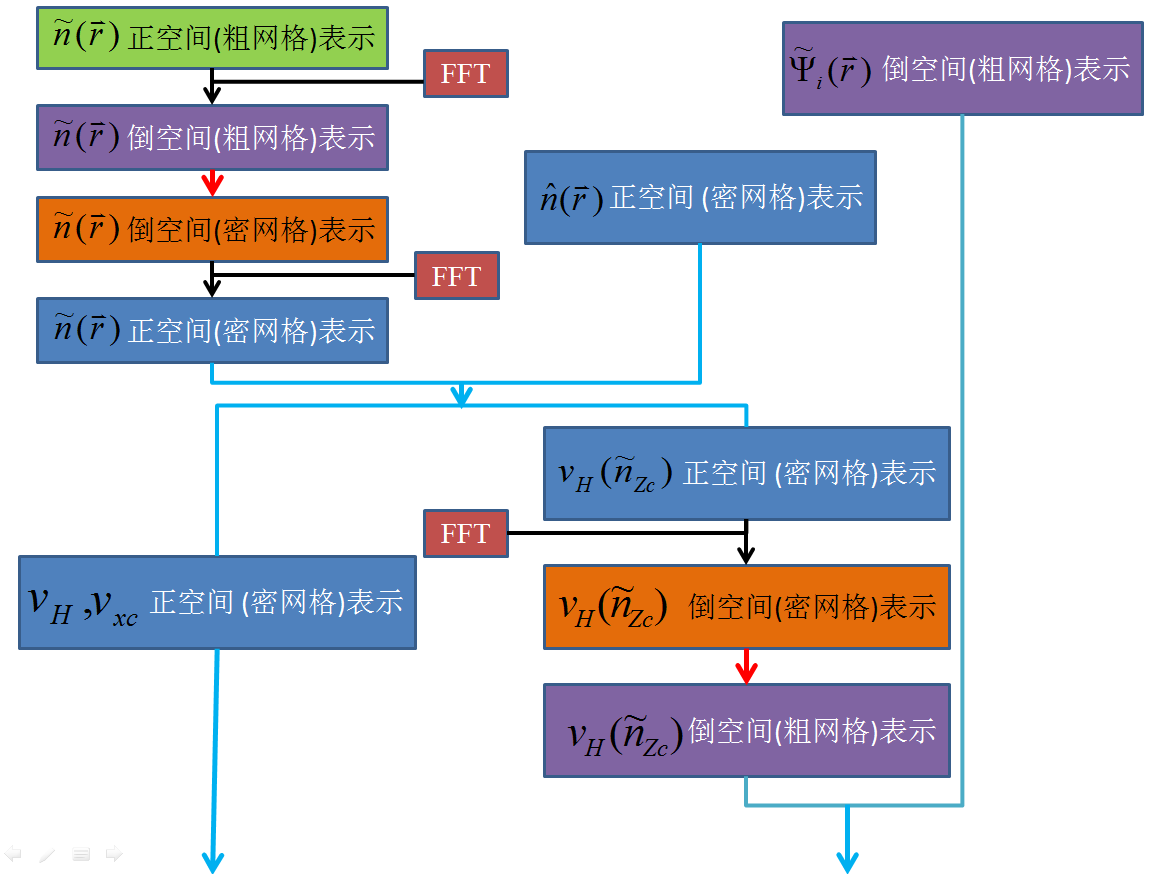
\includegraphics[height=2.7in,width=4.0in,viewport=0 0 1180 875,clip]{Figures/dual_grid.png}
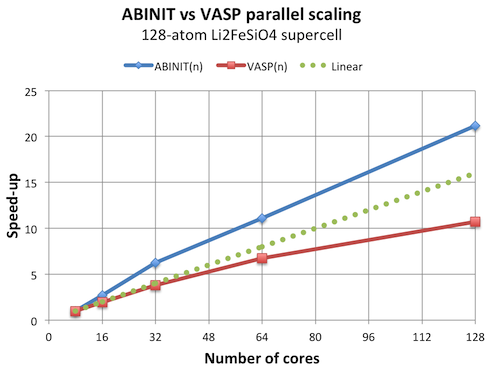
\includegraphics[height=1.55in,width=1.95in,viewport=0 0 240 200,clip]{Figures/VASP-abinit_Li128-1.png}
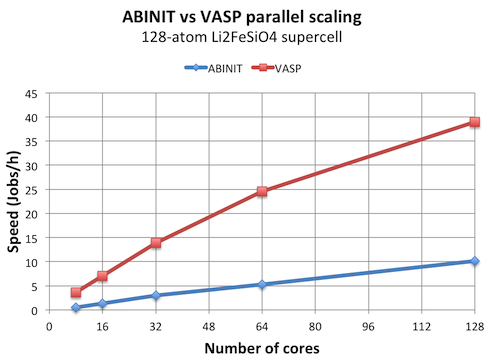
\includegraphics[height=1.55in,width=1.95in,viewport=0 0 240 200,clip]{Figures/VASP-abinit_Li128-2.png}
\caption{\tiny \textrm{The comparison of parallel scaling for ABINIT vs VASP.}}%(与文献\cite{EPJB33-47_2003}图1对比)
\label{ABINIT_vs_VASP}
\end{figure} 
\begin{itemize}
	\item \textrm{VASP}迭代对角化约束了矩阵的维度,减少了对角化过程中的迭代次数,保证了\textrm{MPI}并行的规模和扩展性
	\item \textrm{VASP}实施\textrm{FFT}变换时,保证各节点上处理的网格负载均衡
\end{itemize}
}

\frame
{
	\frametitle{双网格技术}
\begin{figure}[h!]
	\vspace{-0.15in}
\centering
%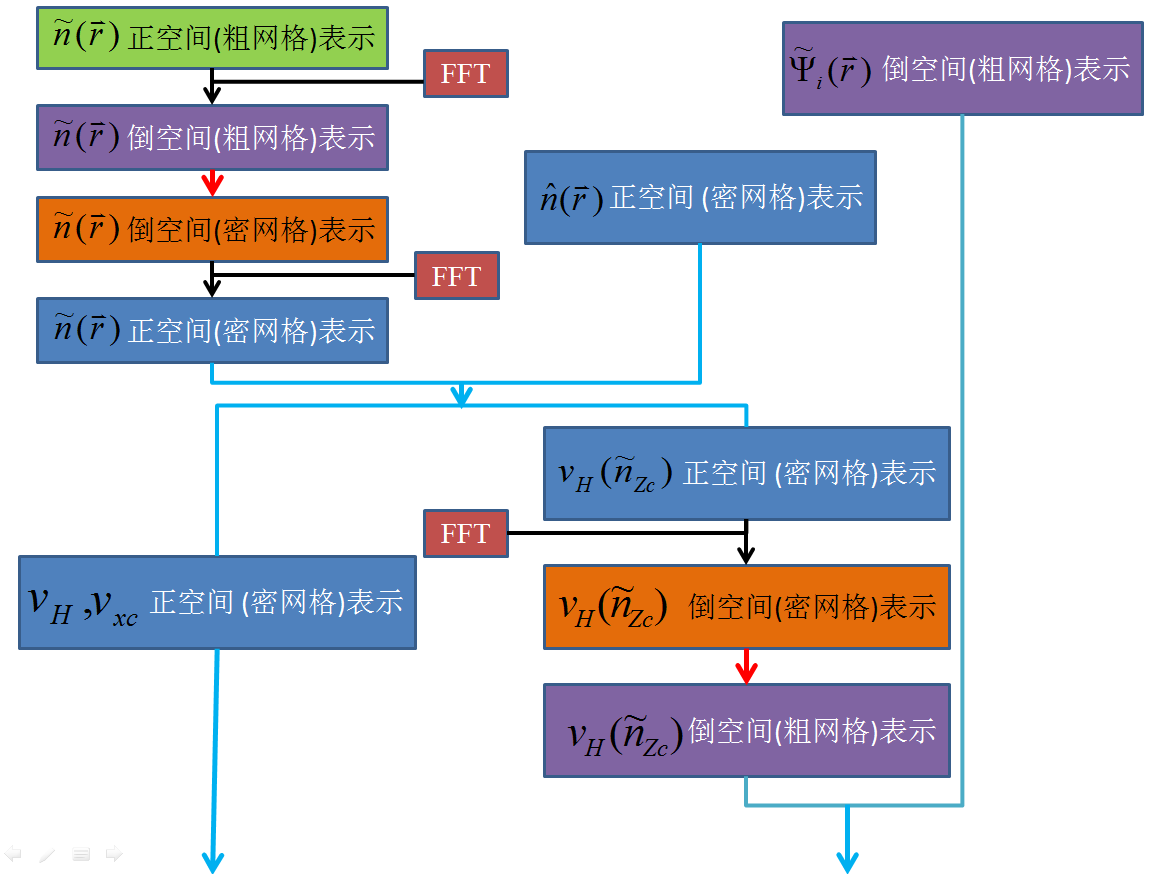
\includegraphics[height=2.7in,width=4.0in,viewport=0 0 1180 875,clip]{Figures/dual_grid.png}
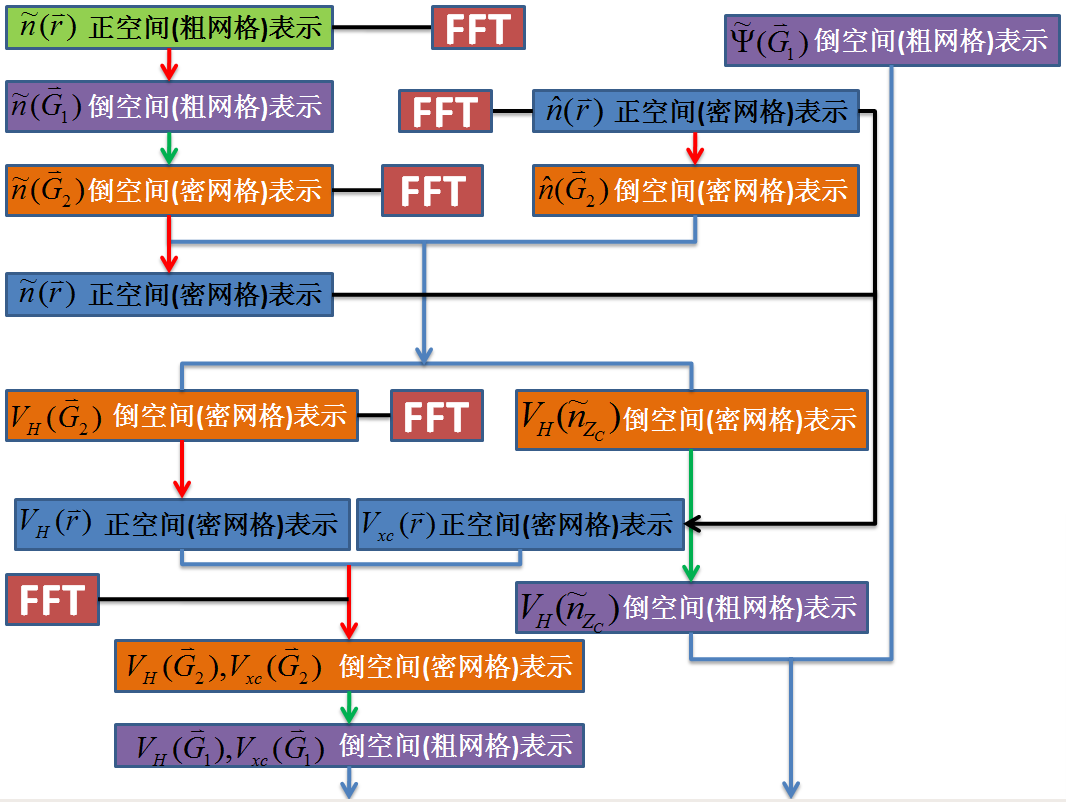
\includegraphics[height=2.75in,width=4.0in,viewport=0 0 800 600,clip]{Figures/dual_grid-2.png}
\caption{\tiny \textrm{The Schematic description of the dual grid technique.}}%(与文献\cite{EPJB33-47_2003}图1对比)
\label{PAW_dualgrid}
\end{figure} 
}

\frame
{
	\frametitle{\textrm{VASP}计算的\textrm{FFT}并行实现}
	\begin{itemize}
	     \item 中间层设计:~\textrm{FFT}网格、实空间基组与计算节点的匹配\\
		     \textcolor{red}{通过子程序\textrm{mgrid.F}生成中间层,实现并行负载与计算节点分配的匹配,减少\textrm{FFT}变换和实空间并行的节点间通信}
\begin{figure}[h!]
		\vspace{-0.25in}
	\centering
%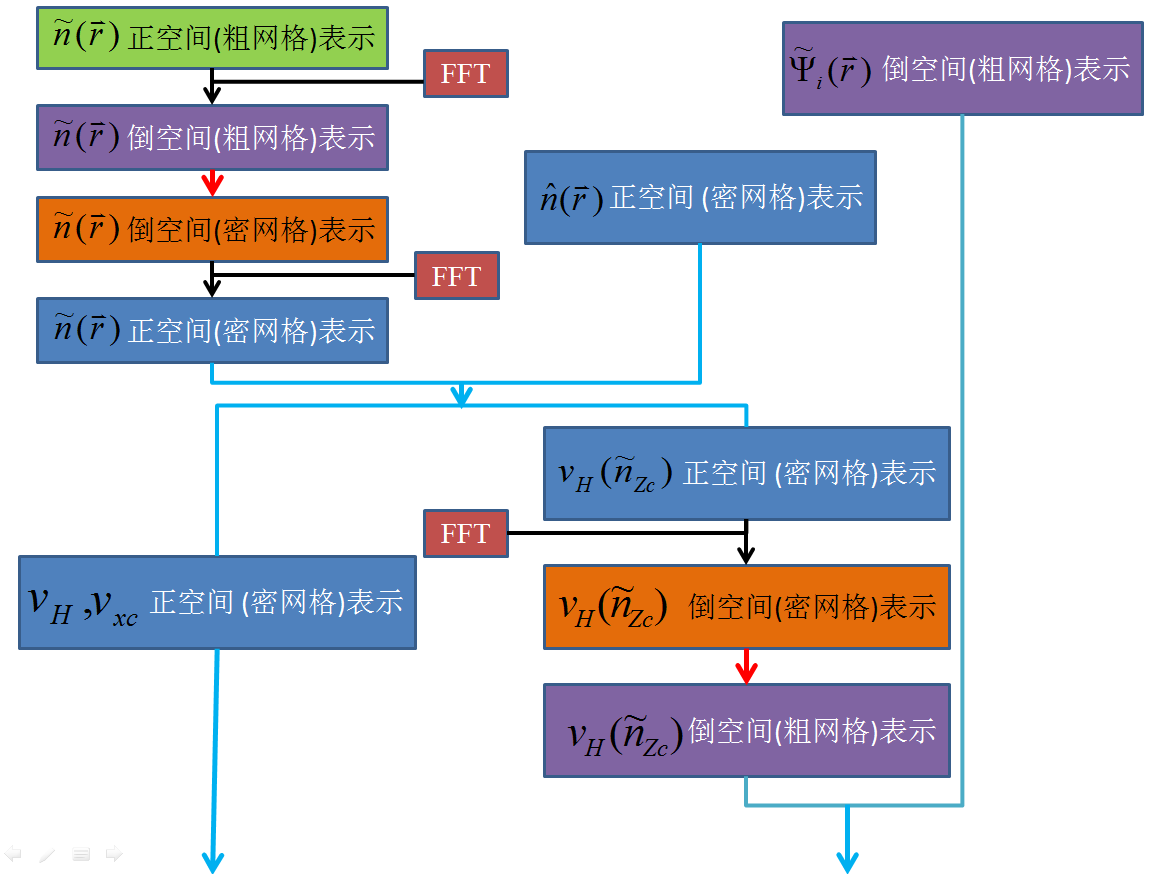
\includegraphics[height=2.7in,width=4.0in,viewport=0 0 1180 875,clip]{Figures/dual_grid.png}
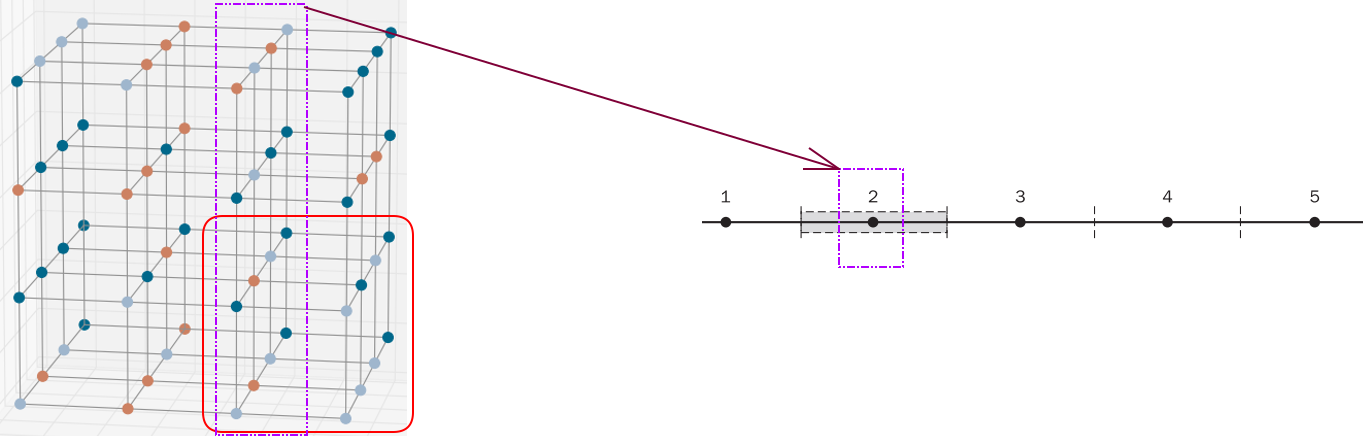
\includegraphics[height=1.0in,width=4.0in,viewport=0 0 1500 450,clip]{Figures/VASP_FFT-MPI_Reciprocal.png}
\vskip 0.5pt
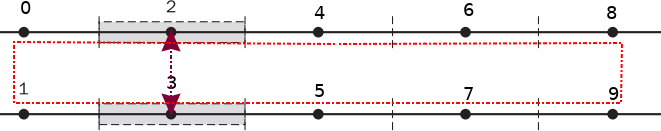
\includegraphics[height=0.7in,width=4.0in,viewport=0 0 730 150,clip]{Figures/VASP_FFT-MPI_Real.png}
\caption{\tiny \textrm{VASP:~ Reciprocal-Real space layout for grids in MPI.}}%(与文献\cite{EPJB33-47_2003}图1对比)
\label{MPI-FFT}
\end{figure} 
	\end{itemize}
}

\frame
{
	\frametitle{\textrm{VASP}的通信开销}
	在高性能的计算队列中,\textrm{VASP}的并行上限可以突破256核,但当并行核数超过百核数量级,并行效率下降非常明显
\begin{figure}[h!]
	\vspace{-0.15in}
\centering
%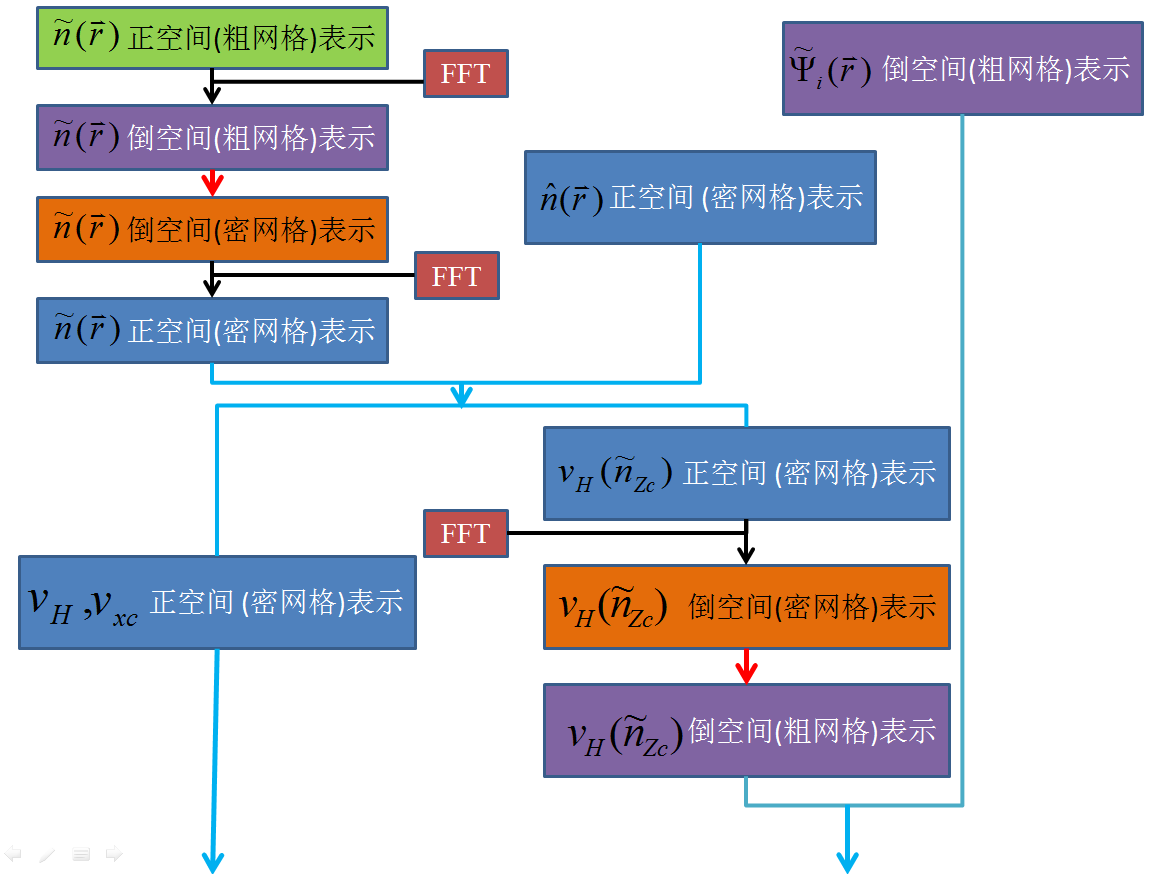
\includegraphics[height=2.7in,width=4.0in,viewport=0 0 1180 875,clip]{Figures/dual_grid.png}
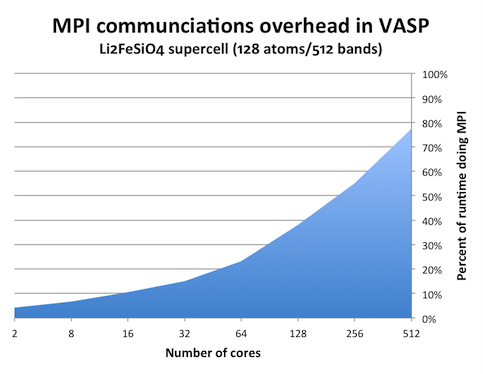
\includegraphics[height=1.55in,width=1.95in,viewport=0 0 240 200,clip]{Figures/VASP-mpi-Li128.png}
\caption{\tiny \textrm{Time spent in MPI calls with increasing the number of ranks in a VASP calculation.}}%(与文献\cite{EPJB33-47_2003}图1对比)
\label{VASP_communication}
\end{figure} 

对并行系统与\textrm{VASP}结合作深度改造(如国家超算天津中心方案),\textrm{VASP}的并行扩展可以到$10^4$核级别,这一改造需要对底层代码和计算框架作较大规模改动
}

\frame
{
	\frametitle{\textrm{VASP}的\textrm{GPU}加速}
\textrm{NVIDIA}多年来致力于\textrm{VASP}的\textrm{GPU}加速,取得了一定的成效
\begin{figure}[h!]
	\vspace{-0.15in}
\centering
%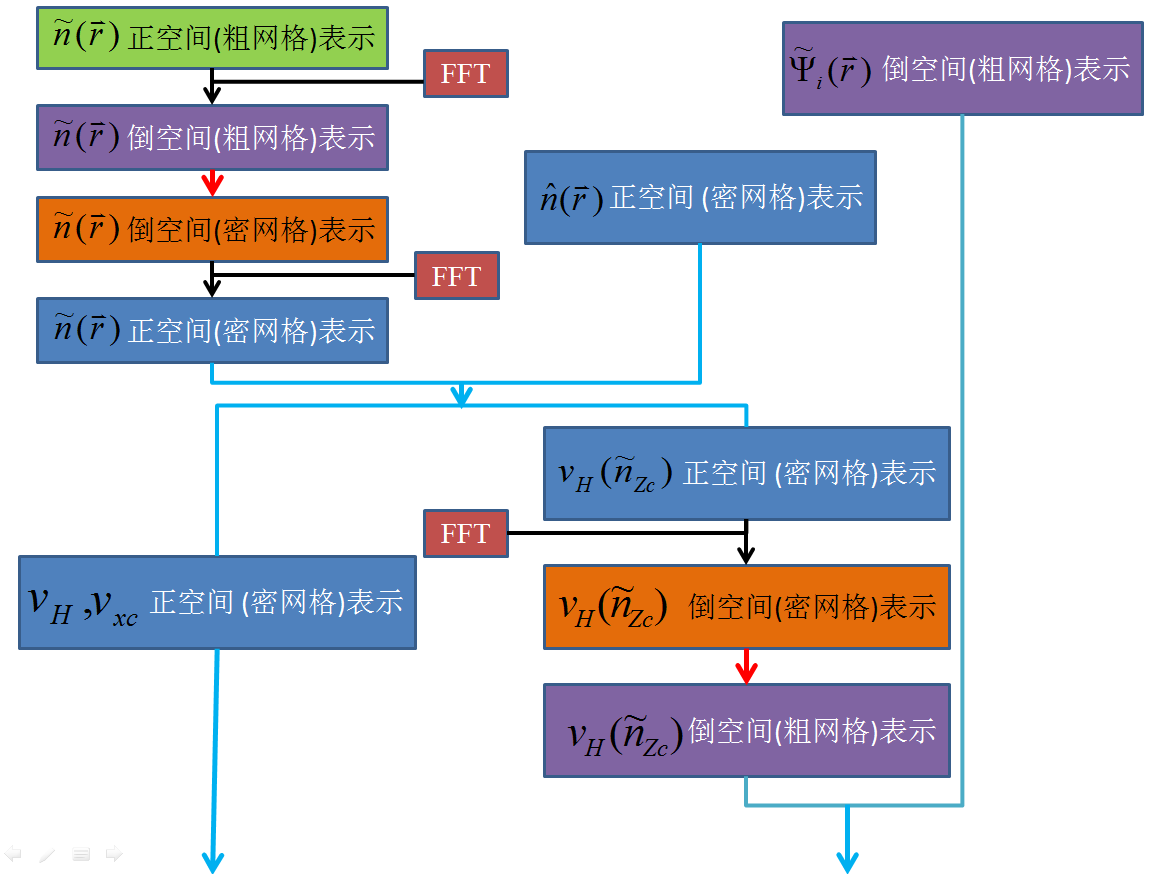
\includegraphics[height=2.7in,width=4.0in,viewport=0 0 1180 875,clip]{Figures/dual_grid.png}
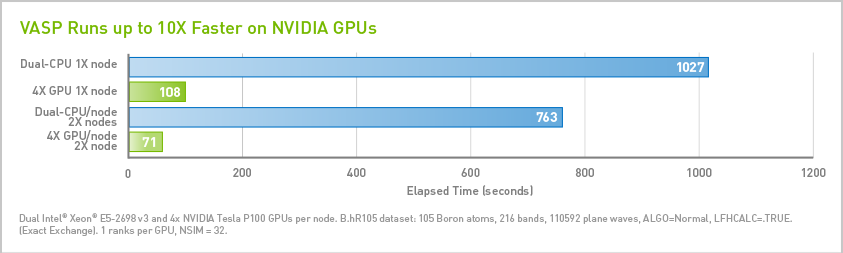
\includegraphics[height=1.2in,width=4.05in,viewport=0 0 850 260,clip]{Figures/VASP-GPU-CPU.png}
\caption{\tiny \textrm{Compare of VASP calculation with GPU and CPU.}}%(与文献\cite{EPJB33-47_2003}图1对比)
\label{VASP_GPU}
\end{figure} 
\begin{itemize}
	\item 通用配置下,\textrm{GPU}对\textrm{VASP}计算有加速效果,一般可提升4$\sim$6倍
	\item 矩阵对角化的并行算法限制了\textrm{GPU}在第一原理计算中的应用
	\item \textrm{GPU}加速的模式主要适合于分子动力学计算
\end{itemize}
}

\section{对\rm{VASP}计算模型扩容}
\frame
{
	\frametitle{对\textrm{VASP}并行优化及计算规模扩容}
	与其余第一原理计算软件相比,\textrm{VASP}的最大优势
	\begin{itemize}
		\item 应用\textrm{PAW}方法,有效处理含有\textit{d}、\textit{f}电子的过渡金属体系
		\item 提供了多种电子结构和原子受力的优化算法(\textrm{SD}、\textrm{CG}、\textrm{RMM-DIIS}等)
		\item 用户可通过控制文件\textcolor{blue}{\textrm{INCAR}}的参数调控来选择
	\end{itemize}
	由于\textrm{VASP}的计算特点,可以处理的模型原子数目的上限一般是百量级($10^2$),对于复杂体系如合金、化合物和电池材料等,现有的模拟规模是制约\textrm{VASP}软件的重要因素
	\vskip 1.5pt
	我们变革了\textrm{VASP}并行方式,%在不改变\textrm{VASP}运行策略基础上
	实现了计算规模的数量级的扩展
\begin{figure}[h!]
\centering
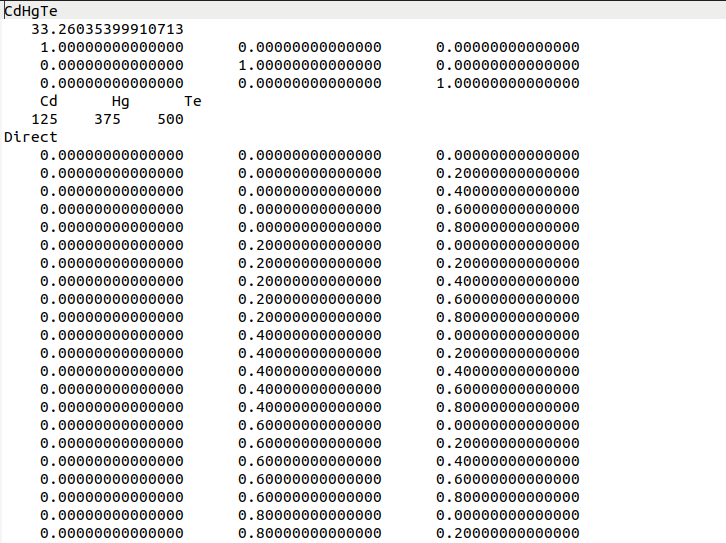
\includegraphics[height=0.85in,width=3.05in,viewport=0 350 726 543,clip]{Figures/VASP_huge_POSCAR.png}
\caption{\tiny \textrm{千原子合金模型.}}%(与文献\cite{EPJB33-47_2003}图1对比)
\label{VASP_Model}
\end{figure} 
}

\frame
{
	\frametitle{计算算例:~控制参数}
\begin{figure}[h!]
\centering
\vskip -0.15in
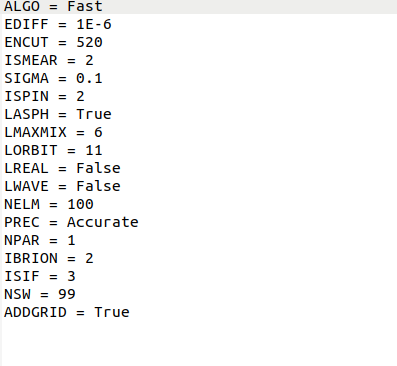
\includegraphics[height=2.75in,width=3.55in,viewport=0 40 397 366,clip]{Figures/VASP_huge_INCAR.png}
\caption{\tiny \textrm{千原子合金模型:~控制参数\textrm{INCAR}.}}%(与文献\cite{EPJB33-47_2003}图1对比)
\label{VASP_Contral}
\end{figure} 
}

\frame
{
	\frametitle{计算算例:~并行规模}
\begin{figure}[h!]
\centering
\vskip -0.15in
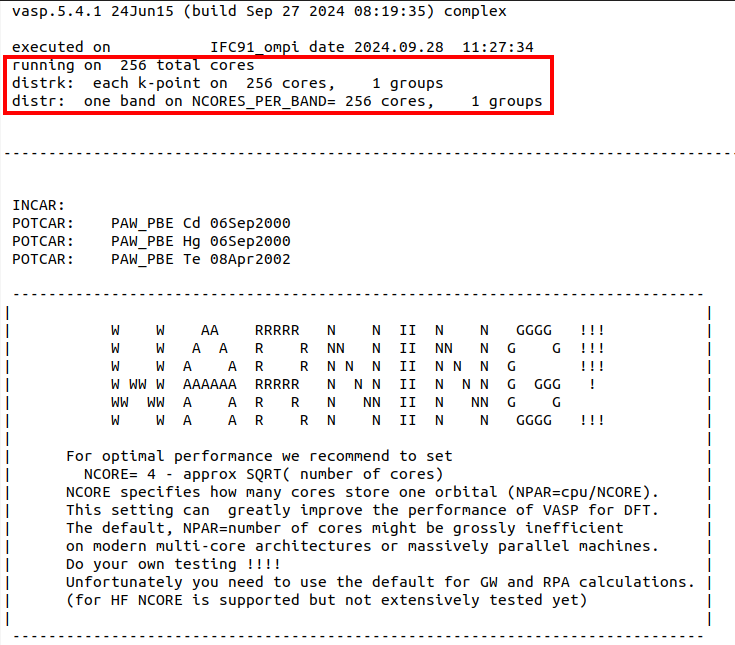
\includegraphics[height=2.75in,width=3.55in,viewport=0 150 735 645,clip]{Figures/VASP_huge_OUTCAR.png}
\caption{\tiny \textrm{千原子合金模型:~并行规模($\vec k$点:~\textcolor{red}{$2\times2\times2$}).}}%(与文献\cite{EPJB33-47_2003}图1对比)
\label{VASP_Parallel}
\end{figure} 
}

\frame
{
	\frametitle{计算算例:~初始计算效率}
\begin{figure}[h!]
\centering
\vskip -0.15in
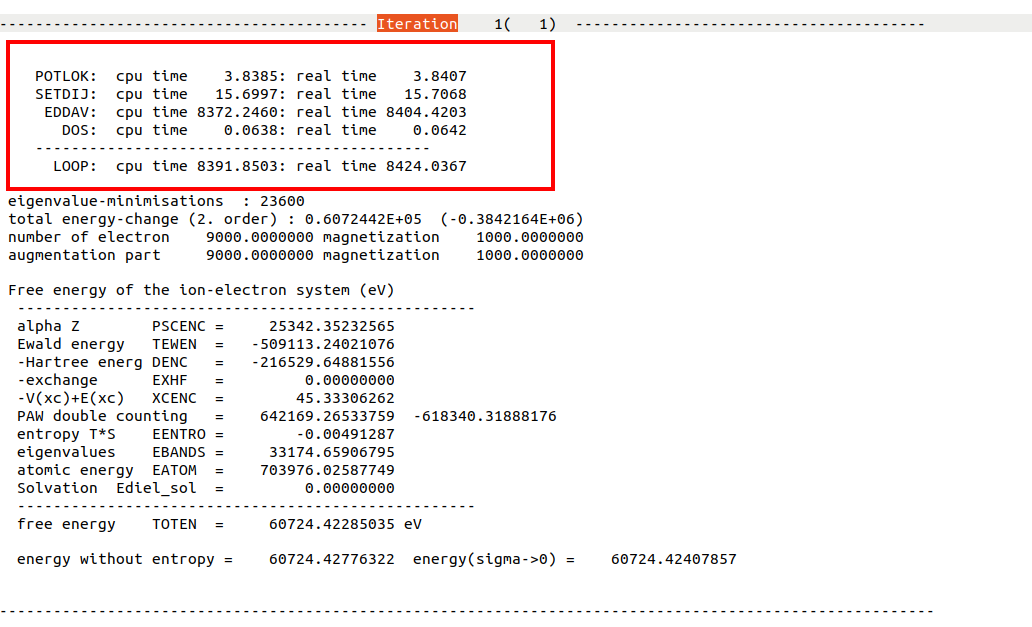
\includegraphics[height=2.75in,width=4.05in,viewport=0 0 1032 627,clip]{Figures/VASP_huge_Iteration-1_1.png}
\caption{\tiny \textrm{千原子合金模型:~计算效率(初始).}}%(与文献\cite{EPJB33-47_2003}图1对比)
\label{VASP_Effectivity}
\end{figure} 
}

\frame
{
	\frametitle{计算算例:~计算效率}
\begin{figure}[h!]
\centering
\vskip -0.15in
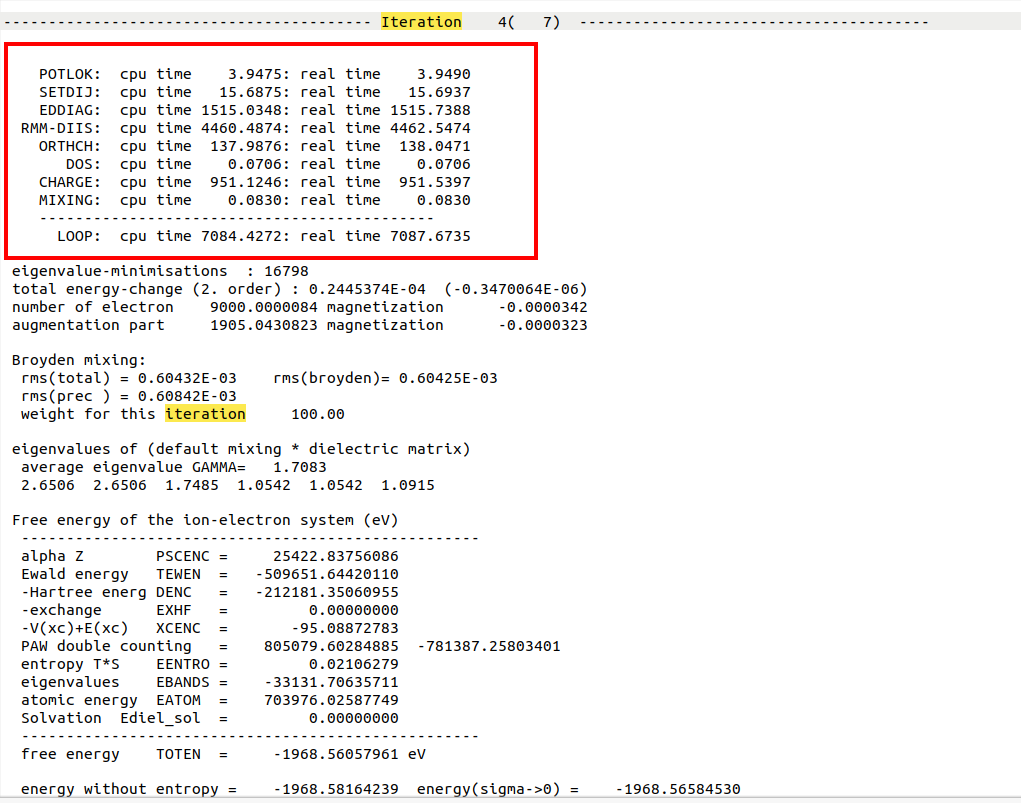
\includegraphics[height=2.75in,width=3.55in,viewport=0 0 1021 803,clip]{Figures/VASP_huge_Iteration-4_7.png}
\caption{\tiny \textrm{千原子合金模型:~计算效率(稳定).}}%(与文献\cite{EPJB33-47_2003}图1对比)
\label{VASP_Effectivity-2}
\end{figure} 
}

\frame
{
	\frametitle{计算算例:~迭代收敛}
\begin{figure}[h!]
\centering
\vskip -0.15in
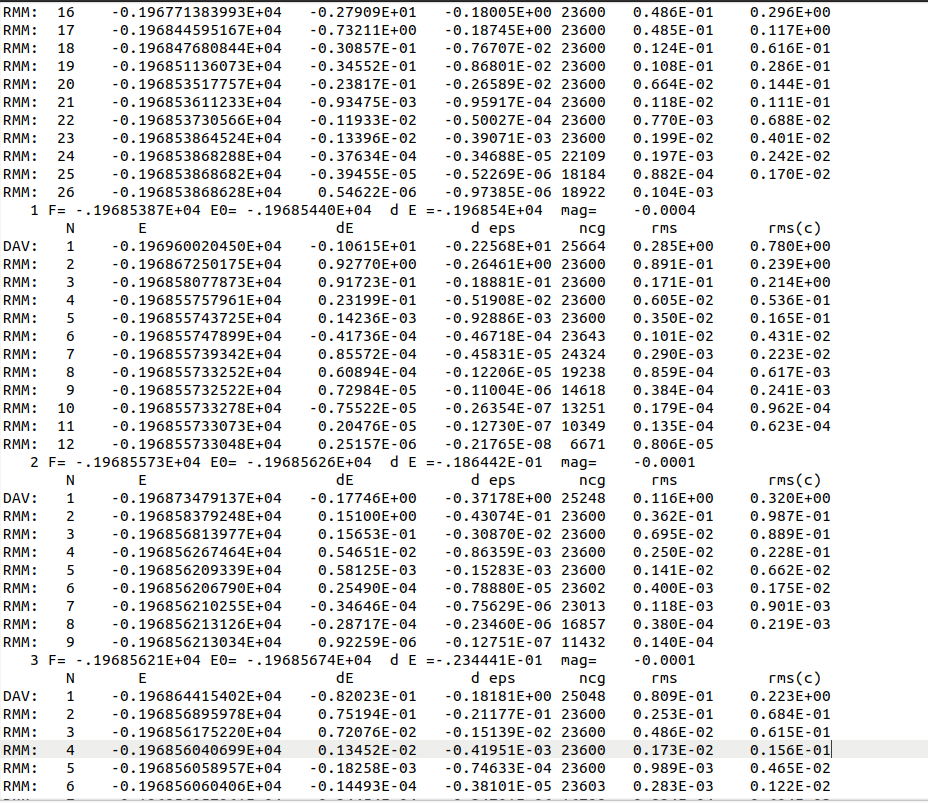
\includegraphics[height=2.75in,width=3.55in,viewport=0 0 928 803,clip]{Figures/VASP_huge_OSZICAR.png}
\caption{\tiny \textrm{千原子合金模型:~迭代收敛.}}%(与文献\cite{EPJB33-47_2003}图1对比)
\label{VASP_Convergence}
\end{figure} 
}

\frame
{
	\frametitle{计算算例}
\begin{figure}[h!]
\centering
\vskip -0.18in
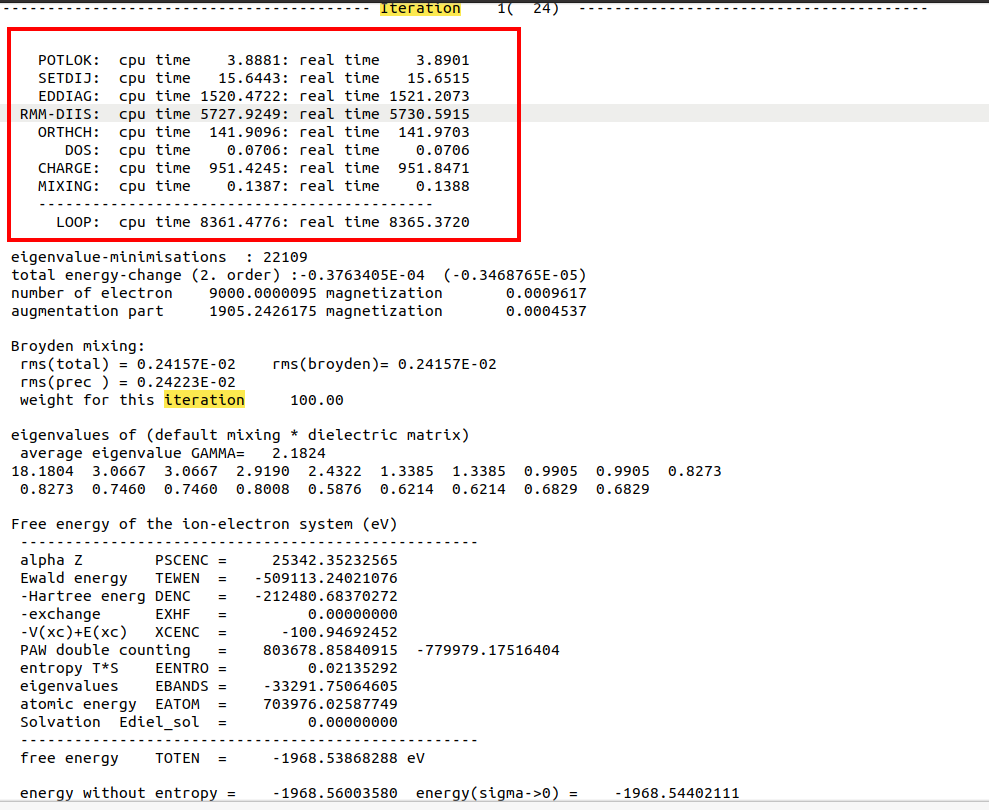
\includegraphics[height=1.35in,width=2.90in,viewport=0 570 589 806,clip]{Figures/VASP_huge_Iteration-1_24.png}
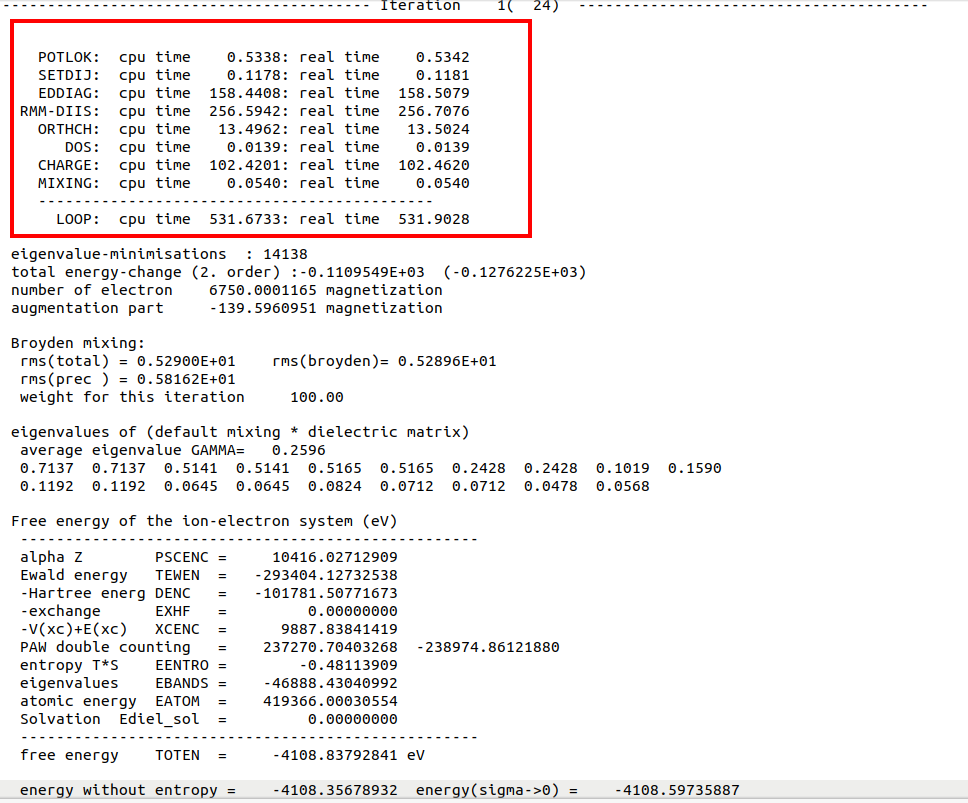
\includegraphics[height=1.35in,width=2.90in,viewport=0 560 568 803,clip]{Figures/VASP_huge_Iteration-1_24-2.png}
\caption{\tiny \textrm{千原子合金模型($\vec k$点:~\textcolor{red}{$2\times2\times2$} vs~\textcolor{red}{$1\times1\times1$}).}}%(与文献\cite{EPJB33-47_2003}图1对比)
\label{VASP_Model-2}
\end{figure} 
}

\section{主要问题}
\frame
{
	\frametitle{软件价值与评估}
	\begin{itemize}
		\setlength{\itemsep}{15pt}
		\item \textrm{VASP}支持的模型至\textcolor{red}{千($10^3$)-万($10^4$)原子量级}\underline{是否必要}
			\vskip 3pt
			{\fontsize{8.2pt}{6.2pt}\selectfont{机器学习势\textrm{(AI)}支持的分子动力学:\\
			是否可以彻底摆脱对第一原理大规模计算\\
		电池材料、高熵合金、超导材料和强关联体系等:\\
	对第一原理计算的模型需求大小}}

		\item \textcolor{blue}{科研用户对千原子量级模型的\underline{计算效率期待}}
		\item 当前\textrm{VASP}支持原子规模的技术方案\underline{是否可行}
	\end{itemize}
}
